\chapter{Экспериментальный раздел}
\label{cha:research}

В данном разделе будет приведены пример работы программы и сравнение времени работы программы.

\section{Примеры работы}
На рисунке \ref{fig:4.1} приведен пример работы программы.

\begin{figure}[h]
    \centering
    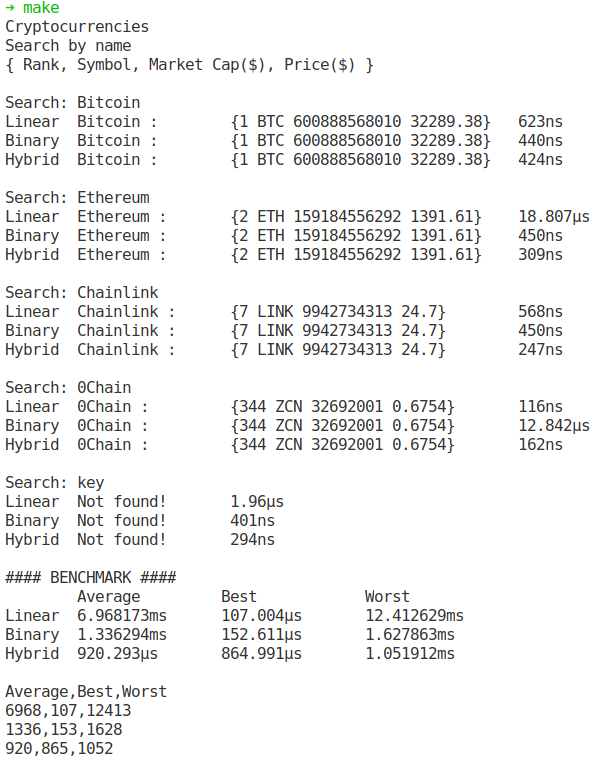
\includegraphics[width=0.8\textwidth]{7/inc/e1.png}
    \caption{Примеры работы программы}
    \label{fig:4.1}
\end{figure}

\section{Результат тестирования}

На рисунке \ref{fig:4.2} приведен результат тестирования.
Словарь состоит из 1000 элементов, были протестированы элементы с номерами 0, 999, 499, 500, 101, 777 и несуществующий ключ.

\begin{figure}[h]
    \centering
    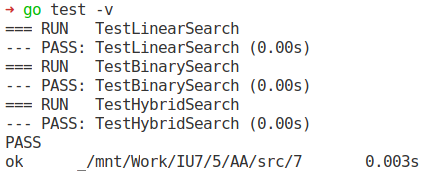
\includegraphics[width=0.6\textwidth]{7/inc/test.png}
    \caption{Результат тестирования}
    \label{fig:4.2}
\end{figure}



% \section{Постановка эксперимента по замеру времени}
% \pagebreak
\section{Сравнение времени работы}

Операционная система - Ubuntu 20.04.1 LTS

Процессор - Intel® CoreTM i5-7300HQ CPU @ 2.50GHz × 4 (ЦП 4 ядра 4 потока)

В таблице \ref{tabular:4.1} приведена таблица частотного анализа.


% \def\arraystretch{1.2}
\setlength\tabcolsep{0.2cm}


\begin{table}[h]
    \centering
    \catcode`\#=12  % deactivate # sign
    \csvreader[tabular=|c|c|,
        table head=\hline
        \bfseries Буква слова
        & \bfseries Количество слов
        \\\hline,
        late after line=\\\hline]
        {7/inc/freq.csv}{}
    { \csvcoli & \csvcolii}
    \catcode`\#=3   % reactivate # sign
    \caption{\label{tabular:4.1} Частотный анализ}
\end{table}


\definecolor{bblue}{HTML}{4F81BD}
\definecolor{rred}{HTML}{C0504D}
\definecolor{ggreen}{HTML}{9BBB59}
\definecolor{ppurple}{HTML}{9F4C7C}

% \clearpage
\begin{figure}[!h]
    \centering
    \begin{tikzpicture}
        \begin{axis}[
            width  = 0.85*\textwidth,
            height = 10cm,
            major x tick style = transparent,
            ybar=2*\pgflinewidth,
            bar width=14pt,
            ymajorgrids = true,
            ylabel = {Время работы, $\mu$с},
            symbolic x coords={Linear,Binary,Hybrid},
            xtick = data,
            scaled y ticks = false,
            enlarge x limits=0.25,
            ymin=0,
            % legend cell align=left,
            % legend style={
            %         at={(1,1.05)},
            %         anchor=south east,
            %         column sep=1ex
            % }
        ]
            \addplot[style={bblue,fill=bblue,mark=none}]
                coordinates {(Linear,6968) (Binary,1336) (Hybrid,920)};
    
            \addplot[style={ggreen,fill=ggreen,mark=none}]
                coordinates {(Linear,107) (Binary,153) (Hybrid,865)};
    
            \addplot[style={rred,fill=rred,mark=none}]
                coordinates {(Linear,12413) (Binary,1628) (Hybrid,1052)};

            \legend{Average,Best,Worst}
        \end{axis}
    \end{tikzpicture}
    \caption{Зависимость времени работы алгоритмов поиска}
    \label{fig:4.4}
\end{figure}

\pagebreak
\section{Вывод}

Эксперимент показывает, что в среднем алгоритм линейного поиска худший, а лучший - гибридный алгоритм (сегментация + бинарный поиск).
Алгоритм линейного поиска не требует сортировки данных, но для отсортированных данных он работает очень быстро, чтобы найти первые (например, найти самую популярную криптовалюту).
Гибридный алгоритм может работать даже лучше с большим количеством сегментов, если вместо линейного поиска сегмента мы будем искать с использованием хэш-карты.